% !TeX spellcheck = en_GB

\documentclass[preprint,12pt]{elsarticle}
\usepackage{graphicx,psfrag,epsf}
\usepackage{amsfonts}
\usepackage{mathtools}
\usepackage{amssymb}
\usepackage{amsmath}
\usepackage{longtable}
\usepackage{bigints}
\usepackage{soul}
\usepackage{tikz}
\usepackage{color}

\usepackage{hyperref}
\usepackage[capitalise]{cleveref}
\usepackage{url}
\usepackage{doi}
\usepackage{multicol}
\usepackage{multirow}
\usepackage{subcaption}

\newcommand{\x}{\boldsymbol{X}}
\renewcommand{\b}{\hat{\beta}}
\newcommand{\reals}{\mathbb{R}}
\newcommand{\normal}{\mathcal{N}}
\newcommand{\lexp}{\underline{\text{E}}}
\newcommand{\uexp}{\overline{\text{E}}}

\usepackage{lineno}
\linenumbers

\begin{document}

\begin{frontmatter}

%% Title, authors and addresses
\title{Robust Bayesian Analysis of Causal Inference Problems}
\author[1]{Tathagata Basu\corref{cor1}}
\ead{tathagatabasumaths@gmail.com}
\cortext[cor1]{Corresponding author}
\author[2]{Matthias C.~M.~Troffaes}
\ead{matthias.troffaes@durham.ac.uk}
\affiliation[1]{organization={Civil and Environmental Engineering, University of Strathclyde},
            addressline={}, 
            city={},
            postcode={}, 
            state={},
            country={}}
\affiliation[2]{organization={Department of Mathematical Sciences, Durham University},
            addressline={South Road}, 
            city={Durham},
            postcode={DH13LE}, 
            %state={},
            country={United Kingdom}}

\begin{abstract}
%%% MT to TB: will try reduce abstract length slightly        
Causal inference using observational data is important in
many fields, including epidemiology, social science, economics, and many more.
The goal of causal inference is to find the treatment effect on the subjects
by identifying causal links between the variables and the outcome.
However, estimation of such causal links is extremely 
difficult because the treatment effects may vary from subject 
to subject. Unfortunately, modelling the underlying heterogeneity explicitly makes the 
problem practically unsolvable. Additionally, for high dimensional problems,
we often need to find a subset of 
explanatory variables to initiate the treatment. However, current variable selection methods
simply tend to maximise the predictive performance of the outcome model. This can be problematic when information and data are limited,
as the consequence of mistreatment can be harmful. 
So, in this paper, we develop a model for causal inference using
robust Bayesian analysis, to allow for abstention when selecting
explanatory variables.
Our robust Bayesian model uses a set of spike and slab priors 
through prior elicitation to obtain robust estimates for
both the treatment and outcome model. We are specifically interested 
in the sensitivity of the treatment effect in the high dimensional causal inference
as well as identifying confounder variables. However, indicator
based confounder selection can be deceptive, especially
when the predictor is strongly associated with either the treatment or 
the outcome, as this increases the posterior expectation of the selection
indicators. To avoid that, we apply a post-hoc selection scheme
which successfully removes negligible non-zero effects from the model,
attaining a smaller set of confounders. Finally, we illustrate
our method using a synthetic dataset.
\end{abstract}

\begin{keyword}
  high dimensional data\sep variable selection\sep Bayesian analysis\sep imprecise probability
\end{keyword}

\begin{highlights}
\item *** TODO ***
\item *** TODO ***
\end{highlights}

\end{frontmatter}

%%% MT to TB: do we say "treatment effect" or "causal effect"? later
%%% in the text both are used; we should pick something and be
%%% consistent to avoid confusion (if indeed they are the same...)

\section{Introduction}\label{sec:intro}

Causal inference concerns estimating the causal
effect of independent variables on a dependent variable. Ideally,
randomised trials are the most efficient way to perform this task.
However, this is not always practical due to, for instance, ethical 
concerns, design cost, population size, to name a few. This
leaves us with observational studies
where data is collected though surveys or record keeping. But this
can be problematic in the presence of confounders, which are variables associated with both the treatment and the outcome.
In such cases, we must be extra cautious as we risk
unwanted bias in the treatment effect estimator \cite{rosenbaum83}.
Several authors have tackled the presence of
confounder variables. 
Robins \cite{Robins1986ANA} used a graphical
approach to identify the causal parameters.
Rosenbaum and Robin \cite{rosenbaum1985} suggested a link model to estimate
the propensity scores for all individuals. Subsequently, several other
methods have been proposed based on propensity score matching;
see \cite{winship99,stuart10} for a brief review.

One of the earlier Bayesian approaches to causal inference
can be found in \cite{rubin1978}. More recently,
with the rise of high dimensional data,
Bayesian methodologies have grown in popularity.
Crainiceanu \text{et al.~}\cite{Crainiceanu2008} proposed a bi-level 
Bayesian model averaging based method for estimating the causal 
effect. Wang \text{et al.~}\cite{wang2015} suggested BAC (or, Bayesian adjustment for
confounding),
%%% MT to TB: check next phrase
where an informative prior obtained from
the treatment model is applied on the outcome model for
estimating the causal effect. Several other methods were
proposed to tackle confounders from a Bayesian perspective,
see for instance \cite{Zigler2014,Hahn2018} among others.

In this paper we take inspiration from the approach of Koch \text{et al.~}\cite{koch2020}, who proposed a bi-level spike and slab prior for causal effect 
estimation. They considered a data-driven adaptive approach to
propose their prior which reduces the variance of the causal estimate. 
Our approach is based on
sensitivity analysis, where instead of using a single prior, 
we consider a set of priors \cite{BERGER1990303}. This is particularly 
interesting as in many cases, causal effect estimation can be performed 
through a meta analysis where robust Bayesian analysis 
can be beneficial under severe uncertainty \cite{raices_cruz22}.
Moreover, for some problems 
we have to rely on very limited data to perform our Bayesian analysis and 
inference with a single prior may not be reliable.
%%% MT to TB: I don't quite understand the heteroscedasticity argument;
%%% I added "inference with a single prior" above instead
% in presence of heteroscedasticity within the data.
Instead, we use expert opinion to elicit a set of priors 
based on empirical evidence. 
This allows us to construct the problem of confounder identification 
in a framework where abstention has a relatively positive gain i.e.~
when the cost of further tests/data collection is cheaper than
mistreating a subject.

Our framework considers a set of continuous spike and slab priors 
\cite{ishwaran2005} for confounder identification.
%%% MT to TB: check if you are happy with this next sentence
We thereby construct a Bayesian group LASSO \cite{xu2015} type problem.
To perform sensitivity analysis,
we consider a set of beta priors on the covariate selection 
probability of the spike and slab priors. We use the posteriors of this
covariate selection probability for identifying the confounders. Finally, 
we consider a post-hoc coefficient adjustment method \cite{hahn2015}
to recover sparse estimates associated with either the outcome or the
treatment model. 

The rest of the paper is organised as follows. In \cref{sec:causal}
we give a formal description of the causal estimation problem in the
context of linear regression. \Cref{sec:bayes} is focused on the
Bayesian analysis of causal inference problems, followed by the
motivation of a robust Bayesian analysis along with our proposed decision 
theoretic framework for confounder (variable) selection. In \cref{sec:sim}, 
we provide results of simulation studies under different scenarios 
and show the possible applications in real life problems. Finally, 
we discuss our findings and conclude this paper in \cref{sec:conc}.

\section{Causal Estimation}\label{sec:causal}

\subsection{Regression Model}

Let an observational study on $n$ individuals give us
the outcomes $Y\coloneqq(Y_1, \dots, Y_n)$ along with 
corresponding treatment indicators $T\coloneqq(T_1, \dots, T_n)$.
Regression methods are widely used in causal effect estimation. The
main idea behind these regression methods is to remove the
correlation between the treatment indicator and the error term
\cite{winship99,HECKMAN1985}.

%%% MT to TB: not sure where this text needs to go, omitted for now...

% In theory, both $\mathbb{E}(Y_i\mid T_i=1)$ and $\mathbb{E}(Y_i\mid T_i=0)$ exist.
% However, we cannot observe them simultaneously, since we cannot `treat' and `not treat' the same individual at the same time.

% We rely on the important assumption that the treatment effect
% on the $i$-th subject given that they received the treatment is the same as the (counterfactual) treatment effect when they remain as control \cite{winship99}.

To do so, we rely on $p$ different observed quantities
or predictors denoted by $X\coloneqq$ $[X_1^T, \dots, X_n^T]^T$
where each $X_i\in\mathbb{R}^p$.
Each $X_i$ is treated as a $p$-dimensional row vector,
so $X$ is a $n\times p$ matrix.
Now, let
$\beta \coloneqq (\beta_1$, \dots, $\beta_p)^T$ denote the vector of regression
coefficients
related to the predictors, and $\beta_T$ denote a regression coefficient related to the treatment.
Then we can define a linear model for the outcome
so that
\begin{equation}
	Y_i =  T_i \beta_{T} + X_i\beta + \epsilon_i
\end{equation}
where $\epsilon_i\sim \mathcal{N}(0, \sigma^2)$.

%%% MT to TB: check if you're happy with this paragraph
To decide whether or not to treat a new individual with given predictors,
we are mainly interested in the effect of the treatment on the outcome.
More precisely, the treatment effect of a new individual, indexed as $n+1$,
whose outcome $Y_{n+1}$ is not yet observed, and with observed predictors $X_{n+1}=x_{n+1}$, is defined by:
\begin{align}
  \delta(x_{n+1})
  &\coloneqq\mathbb{E}(Y_{n+1}\mid X_{n+1}=x_{n+1},T_{n+1} =1) - \mathbb{E}(Y_{n+1}\mid X_{n+1}=x_{n+1},T_{n+1}=0)
\end{align}
For our model, due to linearity of expectation, we have that
\begin{align}
  \delta(x_{n+1})
  &=\beta_T+x_{n+1}\beta+\mathbb{E}(\epsilon_{n+1}\mid X_{n+1}=x_{n+1},T_{n+1} =1) \\
  &\quad - x_{n+1}\beta-\mathbb{E}(\epsilon_{n+1}\mid X_{n+1}=x_{n+1},T_{n+1} =0)\\
  \intertext{and because $\epsilon_{n+1}$ is independent from $X_{n+1}$ and $T_{n+1}$,}
  &=\beta_{T}.
\end{align}
Note that, for this model, the treatment effect $\delta(x_{n+1})$
does not depend on the observed value $x_{n+1}$ of $X_{n+1}$.
So, to find the treatment effect, we simply need to estimate $\beta_T$.

To estimate $\beta_T$ from the data $X$, $Y$ and $T$,
especially in the presence of confounders,
we also need to consider the
association between the treatment indicators $T$ and the predictors $X$.
A common choice in the literature is to use a probit link function.
In this way, we can
specify the conditional probability that subject $i$ receives the treatment through a linear model. 
That is, for another vector of regression coefficients 
$\gamma\coloneqq(\gamma_1, \cdots, \gamma_p)^T$ we define
\begin{align}
	P(T_i=1\mid X_i) = \Phi(X_i\gamma)
\end{align}
where $\Phi$ denotes the cumulative distribution function
of a standard normal distribution. To incorporate this probit
link function, we model the $T_i$ as follows \cite{albert93}:
\begin{align}
    T_i^* &= X_i\gamma +u_i \\
    T_i   &= \mathbb{I}(T_i^*>0)
    =
    \begin{cases}
    1 & \text{if }T_i^*>0 \\
    0 & \text{otherwise}
    \end{cases}
\end{align}
where $u_i\sim\mathcal{N}(0,1)$.
%%% MT to TB: not entirely trivial so I added a quick derivation
With this model, indeed
\begin{align}
  P(T_i=1\mid X_i)
  &=P(T_i^*>0)=P(u_i>-X_i\gamma)=1-P(u_i\le -X_i\gamma) \\
  &=1-\Phi(-X_i\gamma)=\Phi(X_i\gamma)
\end{align}

Now, to construct the joint likelihood function, we define an extended
output $2n\times 1$ column vector
$W\coloneqq\left(\begin{smallmatrix}Y \\ T^*\end{smallmatrix}\right)$
and corresponding $2n\times(2p+1)$ dimensional design matrix
\begin{align}
	Z &\coloneqq
        \begin{bmatrix}
           T_1 & X_1 & 0 \\
           \vdots & \vdots & 0 \\
           T_n & X_n & 0 \\
           0 & 0 & X_1 \\
           \vdots & \vdots & \vdots \\
           0 & 0 & X_n
        \end{bmatrix}
        =
	\begin{bmatrix}
		X_O & 0 \\
		0 & X_T
	\end{bmatrix}
\end{align}
where, $X_O \coloneqq [T, X]$ and $X_T \coloneqq X$. Then, considering the assumption of
Gaussian error terms, we have the following likelihood distribution
\begin{align}
	W\mid Z, \beta_T, \beta, \gamma, \sigma^2 \sim\normal\left(Z\nu, \Sigma\right)\label{eq:like:group},
\end{align}
where $\nu \coloneqq (\beta_T, \beta^T, \gamma^T)^T$ and
\begin{align}
	\Sigma &\coloneqq
	\begin{bmatrix}
		\sigma^2{I}_n & 0 \\
		0 & {I}_n
	\end{bmatrix}.
\end{align}


\section{Bayesian Causal Estimation}\label{sec:bayes}

The likelihood given by \cref{eq:like:group} gives us
a foundation for a Bayesian group LASSO 
\cite{xu2015} type model. This way, we can look into the posterior selection
probability of each predictor. There are several
ways to construct spike and slab priors for
variable selection. Here, we consider a continuous type
\cite{ishwaran2005} prior for faster posterior
computation.


\subsection{Hierarchical model}

Let $\pi_j$ denote the prior probability that the $j$-th
predictor is associated with the outcome or the 
treatment. That is, conceptually,
\begin{equation}
	\pi_j \coloneqq P\left((\beta_j,\gamma_j)\not=(0,0)\right).
\end{equation}
Practically, we model this by defining the following hierarchical model
%%% MT to TB do you mean "from" instead of "for"? for now removed as confusing
% for spike and  slab group LASSO
so that,
for $1\le j\le p$,
\begin{align}
	(\beta_j,\gamma_j)^T \mid \pi_{j}, \sigma^2 &\sim 
	\pi_{j}\normal\left( \begin{bmatrix}
		0 \\
		0
	\end{bmatrix}, 
	\tau_1^2\begin{bmatrix}
		\sigma^2 & 0 \\
		0 & 1
	\end{bmatrix}\right)
	+ (1-\pi_{j}) \normal\left(\begin{bmatrix}
		0 \\
		0
	\end{bmatrix}, 
	\tau_0^2\begin{bmatrix}
		\sigma^2 & 0 \\
		0 & 1
	\end{bmatrix}\right)\\
	\beta_T\mid \sigma^2 &\sim \normal\left(0, \sigma^2\right)\\
        \frac{1}{\sigma^2}&\sim \text{Gamma}(a, b)\\
        %%% MT to TB: text referred to q_j so I changed q -> q_j here
	\pi_{j} &\sim\text{Beta}\left(sq_j, s(1-q_j)\right).
\end{align}
In the hierarchical model, we fix sufficiently small $\tau_0$
$(1\gg\tau_0>0)$ so that  $(\beta_j, \gamma_j)$ has its probability mass 
concentrated around zero. Therefore, this represents the spike component of our prior specification. 
For the slab component, we consider $\tau_1$ to be large so that $\tau_1\ge 1$. This allows the prior for $(\beta_j,\gamma_j)$ to be flat beyond the spike component at the origin. 
We illustrate the components of a bivariate spike and slab prior in 
\cref{fig:ssbl} (with fixed $\sigma=1$). We generate the spike component 
with $\tau_0=0.001$ and the slab component with $\tau_1=5$.

\begin{figure}[h]
	\begin{center}
		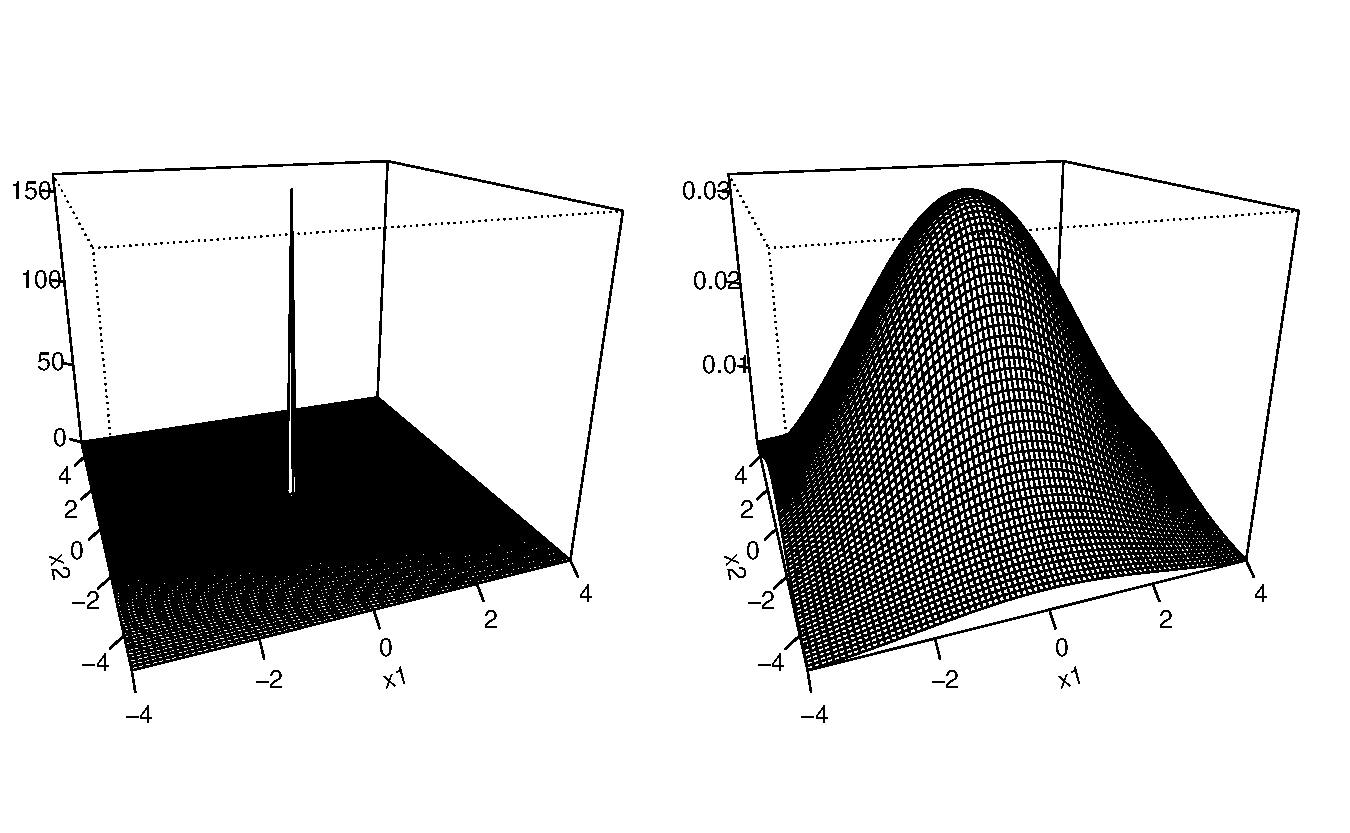
\includegraphics[width = 0.95\linewidth]{spike_slab_bi.pdf}
	\end{center}
	\caption{Spike (left) and slab (right) components of a bi-variate distribution for $\tau_0 = 0.001$, $\tau_1$ = 5 and $\sigma=1$.}
	\label{fig:ssbl}
\end{figure}

For the precision term $1/\sigma^2$, a natural choice of prior is the gamma distribution
as it allows the control of both the location and the scale of the precision.
To ensure that the prior is able to represent the data, we consider $b=1$ and 
fix $a$ so that it represents the prior mean of the precision.
%%% MT to TB: check if you are happy with this
Alternatively, when $b=1$, we know that the interval
$[0, 3a]$ contains the true value of the precision parameter with probability $0.95$.
So, we can also use a prior judgement on the 95\% quantile to set $a$.
We use a beta prior to
model our uncertainty about
the selection probabilities $\pi_j$ where  $q_j$ represents our prior expectation of $\pi_j$ and $s$ acts as 
a concentration parameter.
For the causal effect, we want to use a Gaussian distribution that 
matches the scale of the noise term. Therefore, we consider $\beta_T\sim \normal(0,\sigma^2)$. 

In \cref{fig:regress}, we show a probabilistic graphical representation
of our hierarchical model. In the figure, grey circular nodes represent the
prior hyper-parameters which will be used for sensitivity analysis
of the model. The transparent circular nodes are used to denote
the modelling parameters which are our quantities of interest. 
The observed quantities are denoted with transparent rectangular
nodes. We also use a grey rectangular node to denote the intermediate
latent variable $T^*$. We use directed edges to denote the
relationship between different nodes. However, we use a dashed
edge between $X$ and $T$ as they are related through the latent
variable $T^*$. 

\begin{figure}
	\centering
	\begin{tikzpicture}[params/.style={circle, draw=black!60, very thick, minimum size=7mm},
		hyper/.style={circle, draw=black!60, fill=black!20, thick, minimum size=7mm},
		post/.style={circle, draw=black!60, fill=green!20, thick, minimum size=7mm},
		latent/.style={rectangle, draw=black!60, fill=black!10, dashed, minimum size=7mm},
		data/.style={rectangle, draw=black!60, thick, minimum size=8mm}]
		\node[params] (1) at (0,0) {$\pi$};
		\node[data] (2) at (3,0) {$X$};
		\node[data] (3) at (6,0) {$T$};
		\node[params] (4) at (1.5,1.5) {$\gamma$};
		\node[latent] (5) at (4.5,1.5) {$T^*$};
		\node[params] (6) at (1.5,-1.5) {$\beta$};
		\node[data] (7) at (3.5,-1.5) {$Y$};
		\node[params] (8) at (0,-3) {$\sigma^2$};
		\node[params] (10) at (6,-1.5) {$\beta_T$};
		\node[hyper] (11) at (-1.5,-.8) {$s$};
		\node[hyper] (12) at (-1.5,.8) {$q$};
		\node[hyper] (13) at (-1.5,-2.2) {$a$};
		\node[hyper] (14) at (-1.5,-3.8) {$b$};
		\draw[black, dashed] (0.75,-3.7) rectangle (7,2.1);
		
		\path (1) edge[->]  (6);
		\path (1) edge[->]  (4);
		\path (8) edge[->]  (6);
		\path (6) edge[->]  (7);
		\path (2) edge[->]  (7);
		\path (2) edge[->]  (5);
		\path (5) edge[<-] (4);
		\path (5) edge[->] (3);
		\path (3) edge[->]  (7);
		\path (10) edge[->]  (7);
		\path (2) edge[dashed][->] (3);
		\path (8) edge[bend right = 60][->]  (10);
		\path (11) edge[->]  (1);
		\path (12) edge[->]  (1);
		\path (13) edge[->]  (8);
		\path (14) edge[->]  (8);
		
	\end{tikzpicture}
	\caption{Probabilistic graphical representation for causal inference with Bayesian hierarchical model.}
	\label{fig:regress}
\end{figure}

\subsection{Robust Bayesian Analysis}

The hierarchical model presented above is a standard spike and slab model for
variable selection and performs well when we have sufficient data. 
However, especially in the case of causal inference, we do not always have sufficient data. Moreover, 
we also must be cautious about the side effects of a treatment.
Therefore, we are particularly interested in constructing a robust Bayesian framework
for variable selection. In this way, when we are preparing guidelines for treatment, we 
can have the option to ask for more data before reaching any conclusion. To achieve this,
we consider a utility based framework with three possible 
%%% MT to TB: not sure what is meant, subsequent text does not consider "determining a variable"; replace with "scenarios"?
% ways of determining a variable. 
scenarios.

In general, an unsuccessful treatment of a subject can have severe consequences 
which cannot be associated with a suitable loss function. Instead, we
assume that we can always revert any initial mistreatment by further treatments, 
and we can associate a loss function with the cost of further treatments.
So, we will associate two constant loss values $\ell_1$ and $\ell_2$ 
with false positives and false negatives respectively. 
Clearly, false positives will lead to unwanted side effects and
false negatives will lead to mistreatment of the patient. Finally, we associate
a loss value $\ell_3$ for abstention which can be interpreted as the cost of further tests.
Ideally, in most cases, $\ell_3\ll \ell_1,\ell_2$. However, in certain scenarios,
this might not be the case, especially when the condition of a subject deteriorates rapidly
over time.
\iffalse
\begin{table}[h]
    \caption{Losses with respect to different types of variable selection}
    \label{tab:loss:vs}
    \centering
    \begin{tabular}{l||c|c|c}
       &  False Positive & False Negative & Abstention \\
       \hline
       \hline
       Value  &  $\ell_1$ & $\ell_2$ & $\ell_3$
    \end{tabular}
\end{table}
\fi

%%% MT to TB: text above talks about abstaining from treatment; this is quite different from abstaining from selecting a variable
Now, based on this notion of abstaining from selecting a variable, we can perform
a sensitivity analysis over a set of priors on the prior selection probability.
That is, we can consider a set of possible values for $q$ such that
$q\in\mathcal{P}$, where $\mathcal{P} \subseteq \left(0, 1\right)^{p}$.
Here, the equality occurs for the near vacuous case. However, in real-life
situations, performing a robust Bayesian analysis for the near vacuous case is 
not practical. Instead, we incorporate expert elicitation to define our model.
For instance, we can consider $q\in \left[\underline{q}, \overline{q}\right]$
where $p\underline{q}$ and $p\overline{q}$ represent the bounds of the prior expectation on the
total number of variables present in either of the models.

\subsection{Variable selection and coefficient adjustment}
For the co-variate selection, we look into the posterior expectation of $\pi_j$. 
We consider the $j$-th predictor to be removed from both the
treatment and outcome model, if
%%% MT to TB: should we add a subscript q to \mathbb{E} to emphasize the dependence?
\begin{align}\label{eq:vs:remove}
	\uexp (\pi_j\mid W)\coloneqq \sup_{q\in \mathcal{P}} \mathbb{E}(\pi_j\mid W) < 1/2.
\end{align}
Similarly, we consider the $j$-th predictor to be present in at least one of the models, if
\begin{align}\label{eq:vs:sel}
	\lexp (\pi_j\mid W)\coloneqq \inf_{q\in \mathcal{P}} \mathbb{E}(\pi_j\mid W) \ge 1/2.
\end{align}
Otherwise, we consider the variable to be indeterminate,  in which case we abstain from putting
it in any of the models but instead just report a lack of information.

In general, this framework is
%%% MT to TB: self-sufficient sounds a bit strange here, do you mean "sufficient"?
self-sufficient
for variable selection. However, for
model fitting and prediction, we need to evaluate the values 
of the regression coefficients. For that we first need to find the set of active
predictors with respect to our prior expectation of the selection probability $q$.
For any fixed $q$, we define the set $S(q)$ as the set of all variables which are active
in the treatment model or in the outcome model:
\begin{equation}
	S(q)\coloneqq
	\left\{j\colon \mathbb{E}(\pi_j\mid W) \ge 1/2\right\}.
\end{equation}
For sensitivity analysis,
the intersection of $S(q)$ over all $q$ gives us the set of
active variables obtained through \cref{eq:vs:sel}.
Similarly, the union gives us the set of
variables that are not removed through \cref{eq:vs:remove}.
That is:
\begin{align}
    \mathcal{S}_*\coloneqq \left\{j:\lexp (\pi_j\mid W)\ge1/2\right\}
    = \bigcap_{q\in \mathcal{P}}S(q),
    \qquad \mathcal{S}^*\coloneqq \left\{j:\uexp (\pi_j\mid W)\ge1/2\right\}
    = \bigcup_{q\in \mathcal{P}}S(q).
\end{align}
Clearly, $\mathcal{S}_*\subseteq\mathcal{S}^*$.
$\mathcal{S}_*$ represents the set of variables that are sure to be selected,
$\{1,\dots,p\}\setminus\mathcal{S}^*$ represents the set of variables that are sure to be removed, and
$\mathcal{S}^*\setminus\mathcal{S}_*$ represents the set of variables about which we are undecided.
In this way, through sensitivity analysis, our approach incorporates robustness.

Now, for each fixed value of $q$, let $\hat{\beta}_{S(q)}$ be the posterior means 
of the regression coefficients of the outcome model with respect to
the predictors that belong to $S(q)$. Similarly,
let $\hat{\gamma}_{S(q)}$ be the posterior means of the regression
coefficients for the treatment effects. Since we use continuous 
spike and slab priors, these regression coefficients are not sparse.
Moreover, with our variable selection we only determine whether the variable 
is included in at least one of the models. But, we cannot determine a specific 
association. Therefore, to adjust the sparsity of the estimates and understand
the specific association with the treatment/outcome/both, we apply the 
``decoupled shrinkage and selection'' method proposed by \cite{hahn2015}. 
For that, we solve the following adaptive LASSO-type \cite{Zou2006}
problems

\begin{align}
	\hat{\beta}^D_{S(q)} &= 
	\arg\min_{\beta_{S(q)}} \frac{1}{n}\|X_{S(q)}\hat{\beta}_{S(q)}
	- X_{S(q)} \beta_{S(q)}\|_2^2 + \lambda\sum_{j\in S(q)} 
	\frac{|\beta_{j,S(q)}|}{|\hat{\beta}_{j,S(q)}|}
\end{align}
and
\begin{align}
	\hat{\gamma}^D_{S(q)} &= 
	\arg\min_{\gamma_{S(q)}} \frac{1}{n}\|X_{S(q)}\hat{\gamma}_{S(q)}
	- X_{S(q)} \gamma_{S(q)}\|_2^2 + \lambda\sum_{j\in S(q)} 
	\frac{|\gamma_{j,S(q)}|}{|\hat{\gamma}_{j,S(q)}|}
\end{align}
where $q\in \mathcal{P}$.

\iffalse
The DSS method explained
above give us adjusted coefficient estimates for the treatment
and outcome model. However, as result the causal effect estimate
remains the same and modelling with such adjusted sparse effect 
will contribute to the prediction error. Therefore, we need to 
adjust the causal effect estimate as well. Let
\begin{equation}
    \hat{T}^D = \mathbb{I}\left(X_{S(q)}\hat{\gamma}^D_{S(q)} >0\right)
    \quad\text{and}\quad
    \hat{T} = \mathbb{I}\left(X\hat{\gamma}^q >0\right).
\end{equation}
and let $\beta_{T}^D(q)$
be the causal effect after applying `DSS' and $\hat{\beta}_{T}(q)$ be the
posterior estimate of the causal effect for any fixed $q\in\mathcal{P}$. Then
the adjusted estimate is given by:
\begin{equation}
    \beta_{T}^D(q) = \left(\left(\hat{T}^D\right)^T \hat{T}^D\right)^{-1}
    \left(\hat{T}^D\right)^T \left[\hat{\beta}_{T}(q)\hat{T} 
    + X_{S(q)}\left(\hat{\beta}_{S(q)} - \hat{\beta}^D_{S(q)}\right) 
    +X_{S^C(q)}\hat{\beta}_{S^C(q)}\right]
\end{equation}
where
\begin{equation}
    S^C(q)\coloneqq \left\{1,2,\cdots, p\right\} \neg S(q).
\end{equation}
\fi

\section{Simulation Studies}\label{sec:sim}

For the simulation studies, we consider 2 different settings. In each
case, we generate the design matrix $X$ such that $X_i\sim\mathcal{N}(0, \Sigma)$
for $1\le i\le n$ where $[\Sigma]_{ij} = 0.3^{|i-j|}$. This way, we 
generate 50 predictors for our model with mild correlations among them.
We then use the following generation schemes to generate the outcome and
treatment indicator: 
\begin{equation}
    T_i \sim \text{Bernoulli}\left(1/(1+\exp(-X_i\gamma))\right)
    \quad\text{and}\quad
    Y_i = 4T_i + X_i\beta.
\end{equation}
\begin{description}
    \item[Scenario 1] --- $|\gamma_j|, |\beta_j|>0$ for $j\le 10$
    \item[Scenario 2] --- $|\gamma_j|>0$ for $j\le 10$ and $|\beta_j|>0$ for $j\le 15$
\end{description}
For both
the cases, we consider different numbers of observations $n$ where
$n=25+ 5k$ for $k=0,1,2,\cdots,10$. %depends on finishing
%$n=25\times 2^k$ for $k=0,1,2,\cdots,5$. 

We present our analyses in \cref{tab:causal} and \cref{tab:misspec}.
For the sake of clarity we use the following accronyms: RBCE for 
robust Bayesian causal estimation (our method); SSCE for spike and
slab causal estimation \cite{koch2020}; BSSCE for bi-level spike and slab causal
estimation \cite{koch2020}; and BSSL for Bayesian spike and slab lasso
\cite{xu2015}. As it can be
seen from both the tables, SSCE and BSSCE are formulated for problems
where $p\le n$ and therefore we do not have any results for $n<50$.

\paragraph{Elicitation} For the
elicitation of $\mathcal{P}$, we use marginal correlation between 
$Y$ and $X$ to determine the bounds on number of active variables. We 
set the thresholds to be $0.15$ and $0.35$ for the correlations. We compute the
number of variables with marginal correlation greater than 0.15
(say $p_1$) and number of variables with  marginal 
correlation greater than 0.35 (say $p_2$). 
We use these numbers to obtain the bounds on the number of active
variables so that $\mathcal{P}=[p_2/p , p_1/p]$.

\paragraph{Initialisation} 
To implement our method, we use \texttt{rjags} and for the other three
methods we use the code provided in the appendix of \cite{koch2020}.
For our method, we set $\tau_0=10^{-6}$ and $\tau_1=1$ to construct the
spike and slab prior. For the noise term, we set $a=10$ and $b=1$.  To perform 
our Bayesian analysis with \texttt{rjags}, we first consider an adaptive 
stage with 2000 iterations followed by discarding of 2000 burn in samples 
to refine the posteriors. We consider 5000 MCMC samples to compute the
posterior estimates. For the other methods we use the in-built settings 
to initiate the analyses.

\paragraph{Results}
We provide our result for causal estimate in \cref{tab:causal}. 
As we perform a sensitivity analysis,
our method gives an interval estimate for the causal effect and we show
that in two different rows where the first row gives the lower bound
and the second row gives the upper bound. We notice that our method is 
somewhat in agreement with the other methods but much more consistent
in terms of estimating the treatment effect. However, this is not the
case for other methods and sometimes those methods produce extreme 
values. This can be observed in \cref{fig:comp:trt} as well. Here, the true 
value is represented by the straight line for $\beta_T = 4$. 

From the figure, we can notice that our method tends
to underestimate the causal effect. This suggests that
we may want to have a different value of $a$ for these sets of observations
instead of a fixed value of $a=10$ for all of our analyses.
We can also see that the lower bound tends to improve
with increasing number of observations which validates the assumption that as we accumulate
more information, the interval becomes smaller and converges towards
the true value.

% latex table generated in R 4.3.0 by xtable 1.8-4 package
% Tue May 23 18:29:20 2023
\begin{table}[ht]
\caption{Causal estimates obtained from different methods
for 6 different
numbers of observations.}\label{tab:causal}
\centering
\subcaption*{First scenario: $|\gamma_j|, |\beta_j|>0$ for $j\le 10$}
\begin{tabular}{l|rrrrrrrrrrr}
  \hline
 & 25 & 30 & 35 & 40 & 45 & 50 & 55 & 60 & 65 & 70 & 75 \\ 
  \hline
RBCE (low) & 3.22 & 3.54 & 3.30 & 3.66 & 3.77 & 3.80 & 3.85 & 3.89 & 3.90 & 3.91 & 3.89 \\ 
  RBCE (up) & 4.03 & 3.96 & 3.50 & 3.77 & 3.82 & 3.83 & 3.90 & 3.93 & 3.92 & 3.92 & 3.91 \\ 
  SSCE & -- & -- & -- & -- & -- & 4.24 & 4.11 & 3.99 & 4.00 & 4.00 & 3.99 \\ 
  BSSCE & -- & -- & -- & -- & -- & 4.02 & 4.01 & 4.01 & 4.01 & 4.01 & 4.01 \\ 
  BSSL & -0.23 & 4.07 & 6.80 & 4.05 & 4.00 & 4.00 & 4.01 & 3.98 & 3.99 & 3.99 & 3.99 \\ 
   \hline
\end{tabular}\subcaption*{Second scenario: $|\gamma_j|>0$ for $j\le 10$ and $|\beta_j|>0$ for $j\le 15$}
\begin{tabular}{l|rrrrrrrrrrr}
  \hline
 & 25 & 30 & 35 & 40 & 45 & 50 & 55 & 60 & 65 & 70 & 75 \\ 
  \hline
RBCE (low) & 2.79 & 3.70 & 3.77 & 3.56 & 3.69 & 3.70 & 3.81 & 3.78 & 3.81 & 3.82 & 3.85 \\ 
  RBCE (up) & 3.65 & 4.01 & 3.96 & 3.82 & 3.90 & 3.86 & 3.92 & 3.89 & 3.91 & 3.88 & 3.91 \\ 
  SSCE & -- & -- & -- & -- & -- & 4.80 & 4.05 & 4.06 & 6.02 & 4.04 & 4.04 \\ 
  BSSCE & -- & -- & -- & -- & -- & 10.34 & 8.12 & 4.17 & 4.04 & 4.06 & 4.05 \\ 
  BSSL & -6.68 & 3.62 & 4.06 & 4.07 & 4.06 & 4.02 & 4.05 & 4.07 & 4.03 & 4.05 & 4.04 \\ 
   \hline
\end{tabular}
\end{table}

\begin{figure}
    \centering
    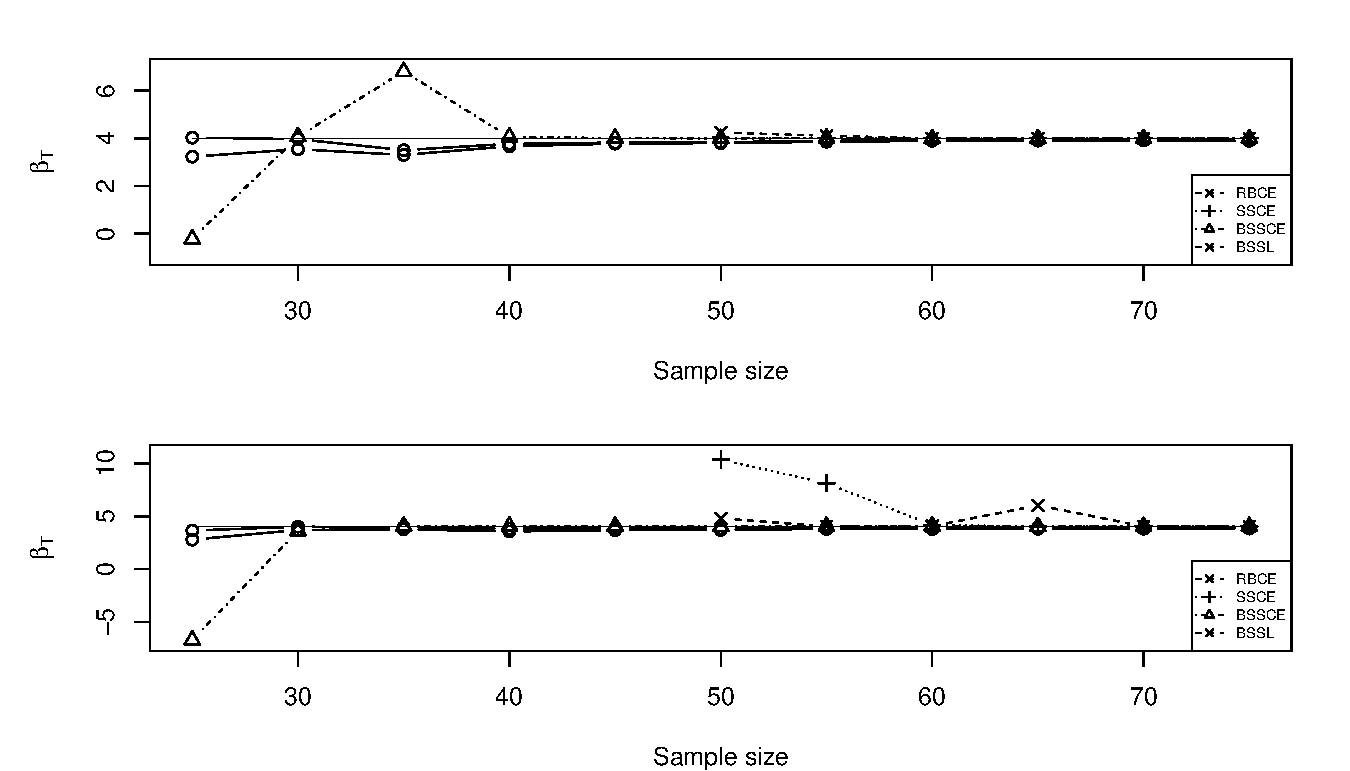
\includegraphics[width = 0.9\linewidth]{RBCE_comp.pdf}
    \caption{Comparison of different methods in estimating the treatment effect.}
    \label{fig:comp:trt}
\end{figure}

For the variable identification, we use the notion of
different losses as described earlier. We consider
$\ell_1=\ell_2 = 1$ and $\ell_3= 0.2$. This is a
simplified way of choosing the loss function, we can choose more 
sophisticated loss functions based on \cite{ZAFFALON20121282}. We use this associated loss
to obtain the total loss, which we present in \cref{tab:misspec}.
In the table we denote the misspecification by counting the number of
false positives (FP) and false negatives (FN). For RBCE, we have an
additional column `ID' which denotes the number of variables which remain as
indeterminate.
From the table it can be seen that for the first scenario, our method
abstains from identifying some variables for 
$n <50$. Especially for $n=25$, our method identifies 26 and 23 variables as indeterminate
for the first setting and second setting respectively. However,
later on our method gives more precise results in terms of variable
selection. We also notice that BSSL tends to perform poorly
in terms of variable selection for $n=25$, this can be seen
from the treatment effect estimation as well.
Moreover, we observe that for the second setting both SSCE
and BSSCE underperform in identifying the active variables, which can 
be explained from \cref{tab:causal} as well. 

% latex table generated in R 4.3.0 by xtable 1.8-4 package
% Wed May 24 00:50:53 2023
\begin{table}[ht]
\caption{Loss based on misspecification of active variables in different
models.}\label{tab:misspec}
\centering
\subcaption*{First scenario: $|\gamma_j|, |\beta_j|>0$ for $j\le 10$}
\begin{tabular}{|c||rrr|r||rr|r||rr|r||rr|r|}
  \hline
  &\multicolumn{4}{c||}{RBCE}&\multicolumn{3}{c||}{SSCE}
  &\multicolumn{3}{c||}{BSSCE}&\multicolumn{3}{c|}{BSSL}\\
  \cline{2-14}
 Samples & FP & FN & ID & Tot & FP & FN & Tot & FP & FN & Tot & FP & FN & Tot \\ 
  \hline
25 &   0 &   0 &  26 & 5.2 & -- & -- & -- & -- & -- & -- &  12 &   2 & 14\\ 
  30 &   0 &   1 &   1 & 1.2 & -- & -- & -- & -- & -- & -- &   0 &   0 & 0\\ 
  35 &   0 &   0 &   1 & 0.2 & -- & -- & -- & -- & -- & -- &   0 &   0 & 0\\ 
  40 &   0 &   1 &   0 & 1.0 &-- & -- & -- & -- & -- & -- &   0 &   0 & 0\\ 
  45 &   0 &   0 &   1 & 0.2 & -- & -- & -- & -- & -- & -- &   0 &   0 & 0\\ 
  50 &   0 &   0 &   0 & 0.0 &  0 &   0  & 0 &   0 &   0  & 0 &   0 &   0  & 0\\ 
  55 &   0 &   0 &   0 & 0.0 &   0 &   0 &   0  & 0 &   0  & 0 &   0 &   0  & 0\\ 
  60 &   0 &   0 &   0 & 0.0 &   0 &   0 &   0 &   0  & 0  & 0 &   0 &   0  & 0\\ 
  65 &   0 &   0 &   0 & 0.0 &   0 &   0 &   0 &   0 &   0  & 0  & 0 &   0  & 0\\ 
  70 &   0 &   0 &   0 & 0.0 &   0 &   0 &   0 &   0 &   0  & 0  & 0 &   0  & 0\\ 
  75 &   0 &   0 &   0 & 0.0 &   0 &   0 &   0 &   0 &   0  & 0  & 0 &   0  & 0\\ 
   \hline
\end{tabular}
\subcaption*{Second scenario: $|\gamma_j|>0$ for $j\le 10$ and $|\beta_j|>0$ for $j\le 15$}
\begin{tabular}{|c||rrr|r||rr|r||rr|r||rr|r|}
  \hline
  &\multicolumn{4}{c||}{RBCE}&\multicolumn{3}{c||}{SSCE}
  &\multicolumn{3}{c||}{BSSCE}&\multicolumn{3}{c|}{BSSL}\\
  \cline{2-14}
 Samples & FP & FN & ID & Tot & FP & FN & Tot & FP & FN & Tot & FP & FN & Tot \\ 
  \hline
25 &   0 &   2 &  23 & 6.6 & -- & -- & -- & -- & -- & -- &   9 &   4 & 13\\ 
  30 &   0 &   2 &   9 & 3.8 & -- & -- & -- & -- & -- & -- &   0 &   0 & 0 \\ 
  35 &   0 &   0 &  18 & 3.6 & -- & -- & -- & -- & -- & -- &   0 &   0 & 0 \\ 
  40 &   0 &   0 &   5 & 1.0 &-- & -- & -- & -- & -- & -- &   0 &   0 & 0 \\ 
  45 &   0 &   0 &   3 & 0.6 & -- & -- & -- & -- & -- & -- &   0 &   0 & 0 \\ 
  50 &   0 &   0 &   1 & 0.2 &  0 &   7 & 7 &   0 &  14 & 14 &   0 &   0 & 0 \\ 
  55 &   0 &   0 &   1 & 0.2 &  0 &   0 & 0 &  0 &  12 & 12 &  0 &   0 & 0 \\ 
  60 &   0 &   0 &   1 & 0.2 &  1 &   0 & 1 &  0 &   0 &  0 & 0 &  0 &   0 \\ 
  65 &   0 &   0 &   0 & 0.0 &  0 &  12 & 12 &  0 &   0 &  0 & 0 &  0 &   0 \\ 
  70 &   0 &   0 &   0 & 0.0 &  0 &   0 &  0 &  0 &   0 &  0 & 0 &  0 &   0 \\ 
  75 &   0 &   0 &   0 & 0.0 &  0 &   0 &  0 &  0 &   0 &  0 & 0 &  0 &   0 \\ 
   \hline
\end{tabular}
\end{table}

\section{Conclusion}\label{sec:conc}

Causal effect estimation is an important tool in statistical learning and needs to
be performed with utmost care as in many cases we may have severe consequence of poor estimation.
In this paper, we tackle this issue by proposing a robust Bayesian analysis of causal 
effect estimation problem for high dimensional data. Our 
framework is focused on the effect of prior elicitation on confounder selection
as well as causal effect estimation. We consider a spike and slab type
prior for confounder selection and discuss the possible sources of uncertainty that
need to be tackled carefully. We were particularly focused on the uncertainty associated
with prior selection probabilities for which we consider a set of beta priors to perform
sensitivity analysis. We showed that the sensitivity analysis on the prior selection probability
gives us a robust confounder selection scheme. In this way, we can abstain from selecting
a confounder when the available data is not sufficient. We also propose a generalised
utility based framework, where we associate a loss for abstaining which can be interpreted 
as the cost of further data collection. Finally, we illustrate our method with synthetic dataset
and compare with other state of the art Bayesian methods. 


Currently, the paper proposes a robust Bayesian approach for causal effect estimation where
we rely on sampling strategies to obtain the posterior bounds as well as performing 
variable selection. In future, it will be interesting to derive inner approximation bounds
for the posterior estimates to reduce the computational cost. Moreover, for the sake of
illustration, we rely on simple loss functions and elicitation strategy. In future, we would
like to investigate different elicitation strategies for the method and explore alternative 
loss functions for formulating a decision theoretic framework. Last but not the least,
we noticed that our method
is in good agreement with other methods with an added level of robustness.
This confirms that our method has good potential for real-life problems,
and we intend to apply it on a real dataset in future work.

\section*{Acknowledgements}

We sincerely thank Jochen Einbeck for his contributions to an earlier version of this paper.

\bibliographystyle{elsarticle-num} 
\bibliography{basu_causal}

\end{document}
